\chapter{Metodi e generazione del dataset}\label{chap:methods_and_materials} % (fold)

\section{Generazione dei Video Sintetici}\label{sec:generazione_dei_video_sintetici}
Come spiegato in \S~\ref{sec:scelta_dataset}, si è deciso di utilizzare il dataset LSMI \cite{kim_large_2021} come punto di partenza per la generazione dei video sintetici, sfruttandone le caratteristiche sopracitate.

Una volta selezionato il dataset di partenza, è stato necessario individuare un processo di generazione che garantisse le seguenti proprietà:

\begin{itemize}
\item \textbf{Riproducibilità}: le trasformazioni applicate a un'immagine devono poter essere replicate in modo deterministico, permettendo di applicare le stesse trasformazioni alla mappa degli illuminanti e alla maschera.
\item \textbf{Credibilità}: il video risultante deve emulare un movimento di camera realistico, comparabile a quello di una ripresa manuale.
\item \textbf{Completezza}: devono essere esplorate sia le regioni a predominanza di un singolo illuminante, sia quelle caratterizzate da illuminanti misti. È inoltre necessario visitare tutti gli illuminanti principali presenti nella scena.
\end{itemize}

\subsection{L'Effetto Ken Burns}
L'approccio adottato si basa sull'effetto \emph{Ken Burns}, reso celebre dall'omonimo regista, che combina pan e zoom per generare un senso di movimento dinamico da immagini statiche. Tale effetto può essere implementato mediante una combinazione di ritaglio (crop) e interpolazione delle coordinate, come illustrato nell'Algoritmo~\ref{alg:Ken_burns_basic}.

\begin{algorithm}[H]
\caption{Effetto Ken Burns base per pan-zoom}
\label{alg:Ken_burns_basic}
\begin{algorithmic}[1]
\Require immagine, fps, durata, zoom\_iniziale, zoom\_finale, dimensioni\_video, direzione
\Ensure sequenza di frame

\State numero\_frame $\gets$ fps $\times$ durata

\For{$i = 0$ \textbf{to} numero\_frame $- 1$}
    \State $t \gets i / (\text{numero\_frame} - 1)$
    \State $\text{zoom} \gets \text{zoom\_iniziale} + t \cdot (\text{zoom\_finale} - \text{zoom\_iniziale})$
    \State Calcola $\text{crop}_w \gets W / \text{zoom}$, $\text{crop}_h \gets H / \text{zoom}$
    
    \If{direzione = orizzontale}
        \State $x_{\text{offset}} \gets t \cdot (W - \text{crop}_w)$
        \State $y_{\text{offset}} \gets (H - \text{crop}_h)/2$
    \ElsIf{direzione = verticale}
        \State $x_{\text{offset}} \gets (W - \text{crop}_w)/2$
        \State $y_{\text{offset}} \gets t \cdot (H - \text{crop}_h)$
    \ElsIf{direzione = diagonale}
        \State $x_{\text{offset}} \gets t \cdot (W - \text{crop}_w)$
        \State $y_{\text{offset}} \gets t \cdot (H - \text{crop}_h)$
    \Else
        \State $x_{\text{offset}} \gets (W - \text{crop}_w)/2$
        \State $y_{\text{offset}} \gets (H - \text{crop}_h)/2$
    \EndIf

    \State Ritaglia l'immagine in base a $(x_{\text{offset}}, y_{\text{offset}}, \text{crop}_w, \text{crop}_h)$
    \State Ridimensiona il crop a dimensioni\_video
    \State Aggiungi il frame alla sequenza
\EndFor

\State \Return sequenza di frame
\end{algorithmic}
\end{algorithm}

\subsection{Punto di Inizio e Fine Parametrico}
Una delle prime modifiche implementate consiste nell'introduzione di parametri espliciti per definire il punto di inizio e il punto di fine del movimento di camera. Questa scelta risponde sia a esigenze di \emph{riproducibilità}, sia di \emph{completezza}.

Il dataset LSMI fornisce, tra i metadati, le coordinate dei color checker presenti in ogni scena. Tali marker sono posizionati intenzionalmente in regioni caratterizzate da elevata predominanza di un singolo illuminante \cite{kim_large_2021}. Lavorando su coppie consecutive di color checker e concatenando video in sequenza, è possibile esplorare sistematicamente tutte le condizioni di illuminazione della scena stessa.

Le coppie di color checker vengono generate in modo circolare: data una scena con $N$ color checker etichettati come $\{c_1, c_2, \ldots, c_N\}$, vengono creati $N$ segmenti video corrispondenti alle coppie $(c_1, c_2), (c_2, c_3), \ldots, (c_{N-1}, c_N), (c_N, c_1)$. Questa strategia garantisce che ogni illuminante venga visitato e che non vi siano discontinuità nel percorso finale, formando un ciclo completo attraverso tutti gli illuminanti della scena.

Un esempio del percorso ottenuto concatenando più video di questo tipo è visibile in Figura~\ref{fig:percorso_video}.

\begin{figure}[ht]
  \centering
  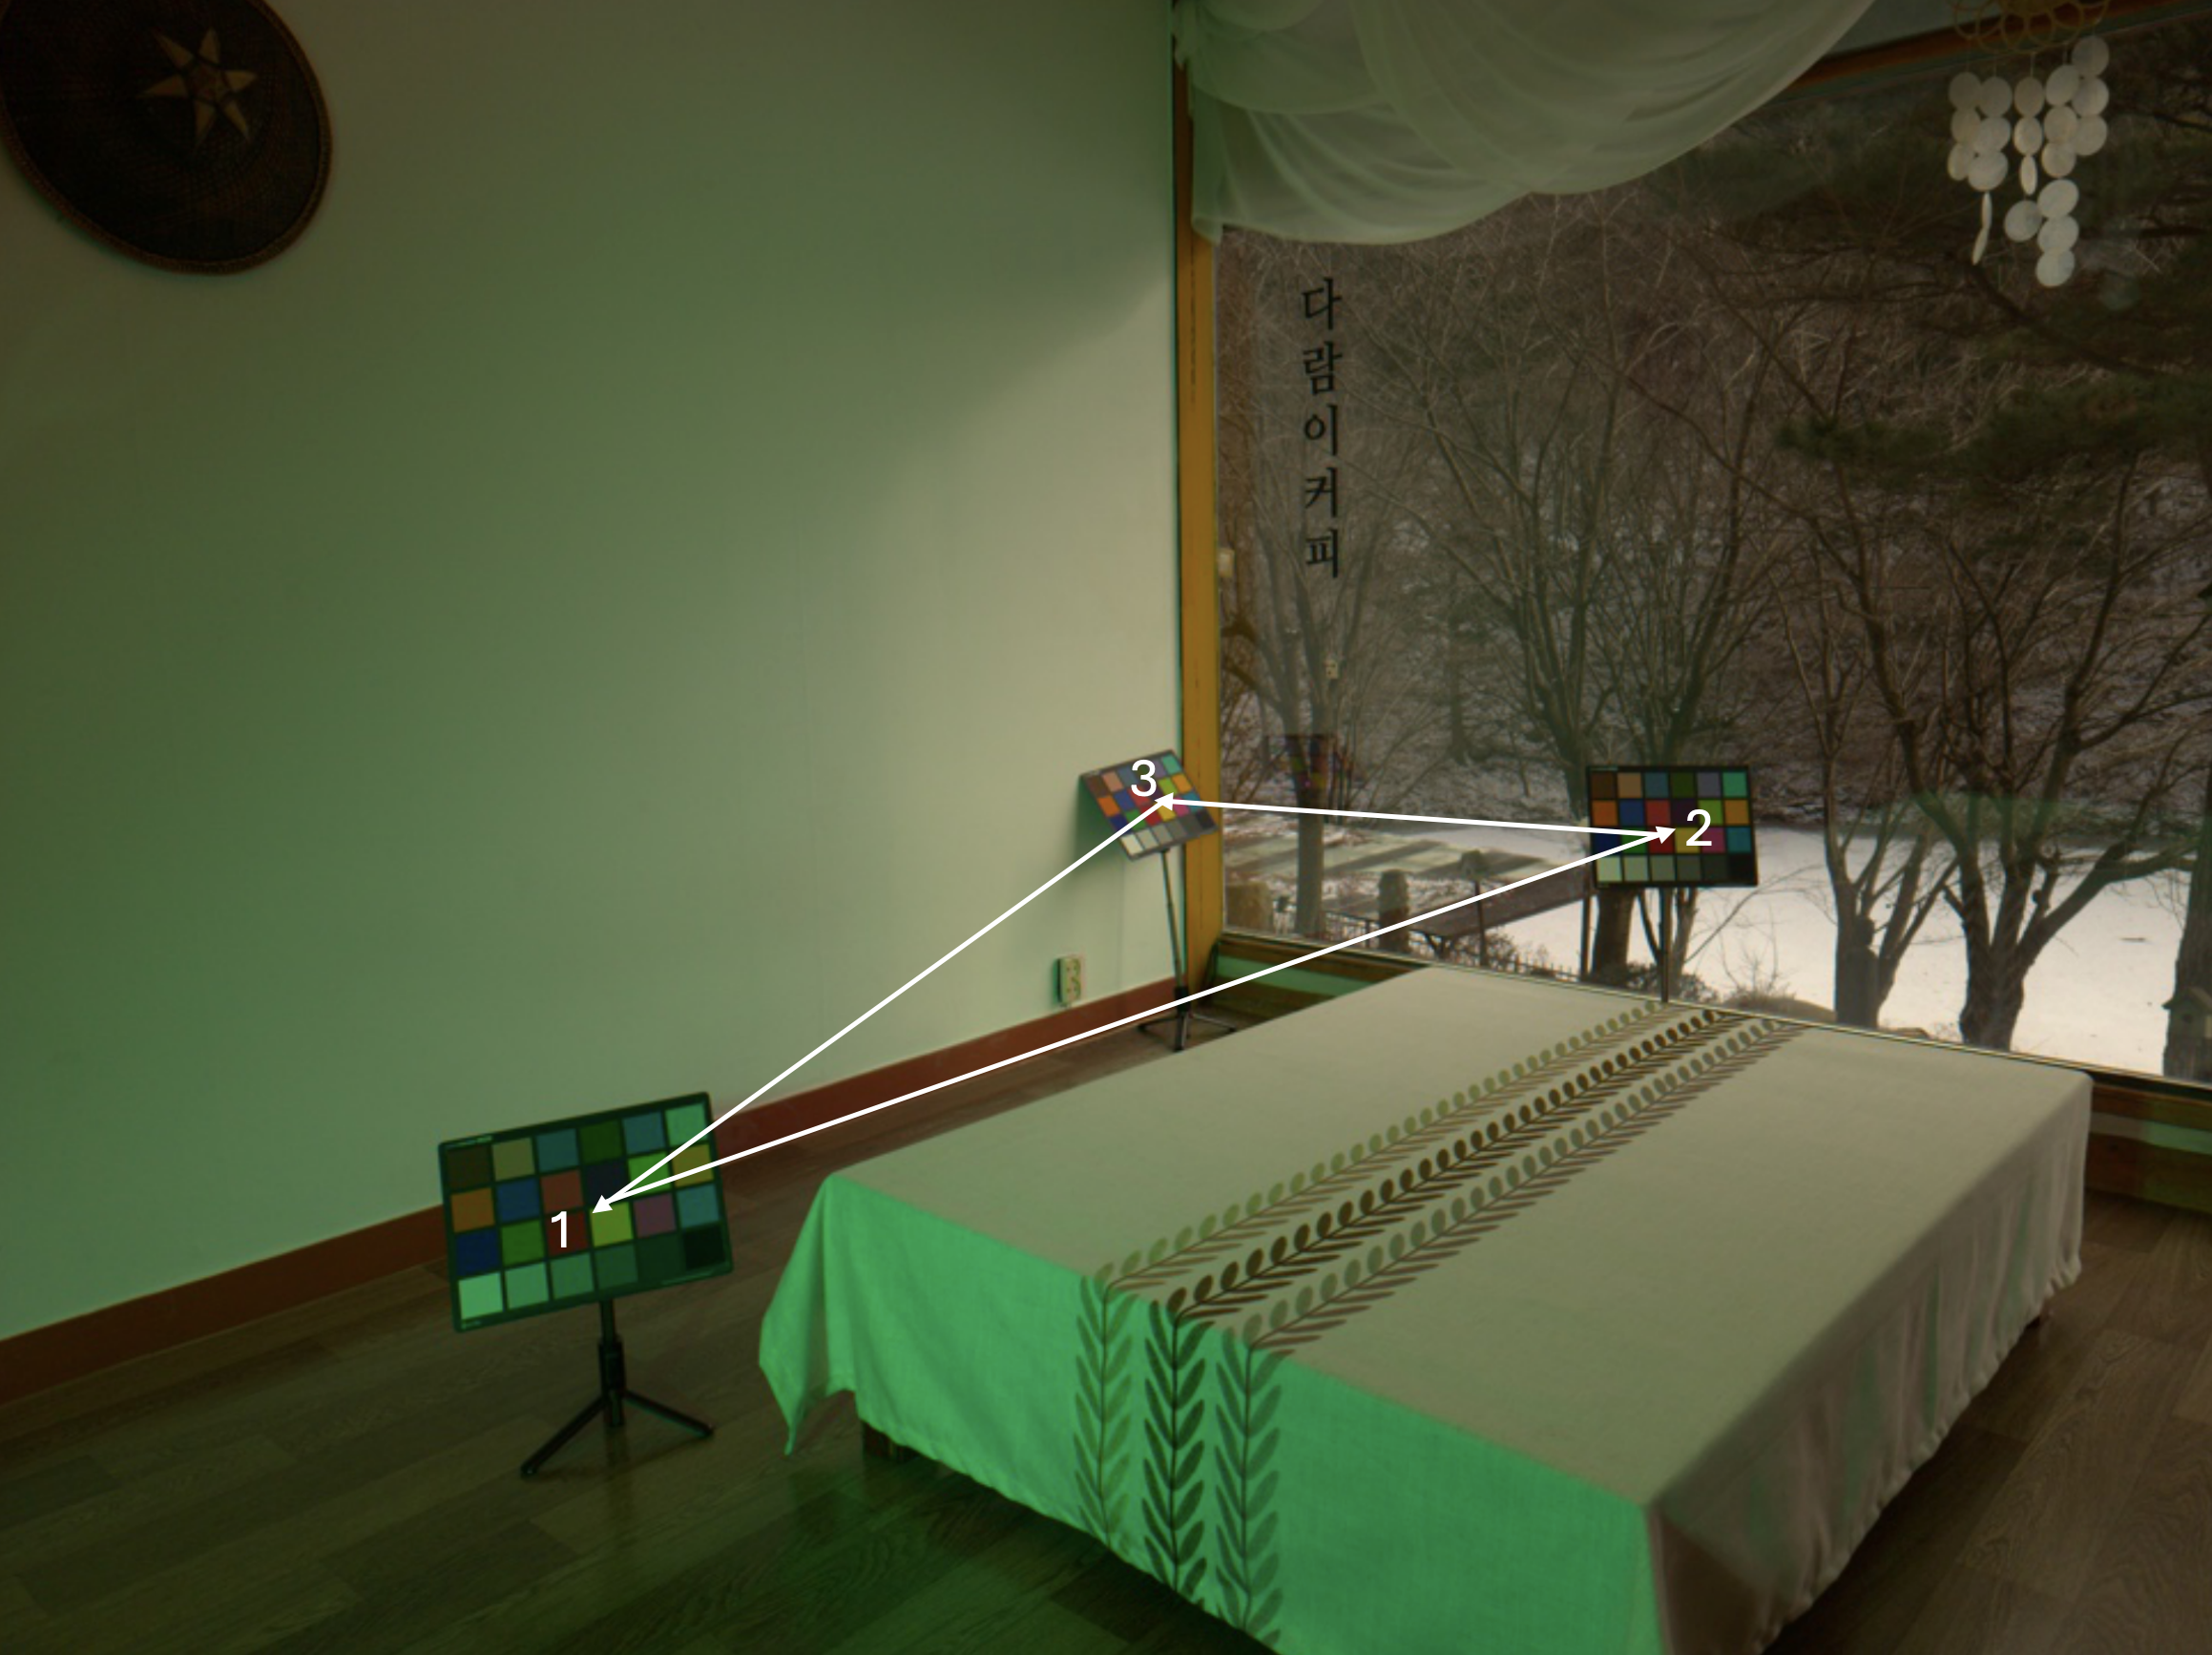
\includegraphics[width=0.8\textwidth]{img/percorso_video.png}
  \caption{Percorso di esplorazione degli illuminanti tramite concatenazione di segmenti video tra coppie di color checker. Ogni segmento connette due marker posizionati in regioni a predominanza di illuminante diversa.}
  \label{fig:percorso_video}
\end{figure}

A livello implementativo, l'algoritmo già utilizza l'interpolazione lineare delle coordinate per il pan. È quindi sufficiente sostituire le coordinate calcolate in base all'offset con quelle fornite esplicitamente come parametri di inizio e fine.

\subsection{Curve di Interpolazione}
Per rendere il movimento tra color checker più naturale e simile a un'effettiva ripresa con camera mobile, si è deciso di esplorare diverse funzioni di interpolazione oltre a quella lineare, la cui equazione è data da:
\begin{equation}
    f_{\text{linear}}(t) = t
    \label{eq:interp_linear}
\end{equation}

Sono state valutate le seguenti parametrizzazioni di $t \in [0, 1]$:

\begin{equation}
    f_{\text{logarithmic}}(t) = \frac{\ln(1 + 9t)}{\ln(10)}
    \label{eq:interp_logarithmic}
\end{equation}

\begin{equation}
    f_{\text{exponential}}(t) = \frac{e^t - 1}{e - 1}
    \label{eq:interp_exponential}
\end{equation}

\begin{equation}
    f_{\text{ease-in-out}}(t) = \frac{1 - \cos(\pi t)}{2}
    \label{eq:interp_ease_in_out}
\end{equation}

La scelta è ricaduta sulla funzione \emph{ease-in-out} \eqref{eq:interp_ease_in_out}, che introduce un'accelerazione graduale all'inizio del movimento e una decelerazione simmetrica verso la fine, generando transizioni più fluide e realistiche.

\subsection{Disturbi Credibili Tramite Perlin Noise}
Per migliorare ulteriormente la \emph{credibilità} del movimento, è stato introdotto un disturbo guidato da \emph{Perlin Noise} \cite{perlin_image_1985}, una forma di gradient noise continua e naturale, ampiamente utilizzata in computer grafica per la generazione procedurale di contenuti.

I valori restituiti dalla funzione di Perlin Noise vengono utilizzati come offset da applicare alle coordinate del centro del frame corrente. La continuità del rumore garantisce l'assenza di discontinuità nel movimento tra frame consecutivi, evitando salti artefatti. La possibilità di specificare un \emph{seed} deterministico consente di replicare la stessa perturbazione su più video, preservando la \emph{riproducibilità} del processo.

\subsubsection{Parametri del Perlin Noise}
L'implementazione del Perlin Noise richiede la definizione di diversi parametri che influenzano le caratteristiche del disturbo applicato:

\begin{itemize}
    \item \textbf{Ampiezza}: controlla l'entità massima dello spostamento in pixel. Un valore tipico utilizzato è compreso tra 5 e 15 pixel, simulando il naturale tremore di una camera tenuta a mano.

    \item \textbf{Frequenza}: determina la velocità di variazione del disturbo nel tempo. Valori di frequenza nell'ordine di $0.1$--$0.3$ producono oscillazioni graduali comparabili a movimenti umani realistici.

    \item \textbf{Ottave}: numero di livelli di dettaglio sovrapposti nel noise. Utilizzando 2--3 ottave si ottiene un disturbo con variazioni sia a bassa che ad alta frequenza, aumentando il realismo del movimento.

    \item \textbf{Seed}: parametro deterministico che permette la riproduzione esatta della stessa sequenza di disturbi, garantendo coerenza tra video \texttt{og}, \texttt{gt}, \texttt{mask} e \texttt{illum}.
\end{itemize}

La combinazione di questi parametri permette di generare un movimento che emula fedelmente le microvariazioni tipiche di riprese manuali, senza introdurre discontinuità percettibili.

\subsection{Gestione dei Bordi}
Durante l'applicazione delle trasformazioni di crop e zoom, combinata con il disturbo introdotto dal Perlin Noise, è possibile che le coordinate del crop risultante eccedano i limiti dell'immagine sorgente. Per preservare la qualità dei video generati ed evitare artefatti visivi, è stata implementata una strategia di gestione dei bordi basata su \emph{clipping} delle coordinate.

Prima di estrarre il crop centrato in $(c_x, c_y)$ con dimensioni $(\text{crop}_w, \text{crop}_h)$, le coordinate vengono vincolate all'interno dei limiti validi dell'immagine:

\begin{align}
    x_{\text{min}} &= \max\left(0, c_x - \frac{\text{crop}_w}{2}\right) \\
    x_{\text{max}} &= \min\left(W, c_x + \frac{\text{crop}_w}{2}\right) \\
    y_{\text{min}} &= \max\left(0, c_y - \frac{\text{crop}_h}{2}\right) \\
    y_{\text{max}} &= \min\left(H, c_y + \frac{\text{crop}_h}{2}\right)
\end{align}

Dove $W$ e $H$ rappresentano rispettivamente la larghezza e l'altezza dell'immagine sorgente. Questa operazione di clipping garantisce che il crop estratto sia sempre valido e completamente contenuto nell'immagine, evitando la necessità di introdurre padding artificiale o bordi neri che comprometterebbero la naturalezza del video.

La strategia adottata è conservativa: nei rari casi in cui il disturbo del Perlin Noise porterebbe il crop oltre i limiti, il movimento viene limitato al massimo spostamento ammissibile. Questa scelta preserva la continuità temporale del movimento senza introdurre discontinuità visive.

\subsection{Pseudocodice del Processo Finale}
L'insieme delle modifiche descritte nelle sezioni precedenti permette di soddisfare tutti i requisiti definiti all'inizio della sezione\S~\ref{sec:generazione_dei_video_sintetici}. L'Algoritmo~\ref{alg:video_generation} fornisce una rappresentazione ad alto livello del processo applicato per la generazione dei video finali.

\begin{algorithm}[H]
\caption{Generazione video sintetico da immagine}
\label{alg:video_generation}
\begin{algorithmic}[1]
\Require immagine, coppie\_centroidi, frame\_totali, zoom, seed
\Ensure video (frame\_totali, $H$, $W$, $C$)

\State $\text{frame\_per\_segmento} \gets \text{frame\_totali} / |\text{coppie\_centroidi}|$
\State Genera seed deterministici per ogni segmento a partire da seed base
\State $\text{segmenti} \gets [ ]$

\For{\textbf{each} (centroide\_inizio, centroide\_fine) \textbf{in} coppie\_centroidi \textbf{with} seed$_i$}
    \State segmento $\gets$ \Call{ArtificialVideo}{immagine, centroide\_inizio, centroide\_fine,  zoom, seed$_i$, frame\_per\_segmento}
    \State Aggiungi segmento a segmenti
\EndFor

\State video $\gets$ \Call{Concatena}{segmenti lungo l'asse temporale}
\State \Return video

\vspace{0.5em}

\Function{ArtificialVideo}{img, start, end, zoom, seed, n\_frames}
    \State Inizializza generatore Perlin Noise con seed
    \State frames $\gets$ array vuoto (n\_frames, $H$, $W$, $C$)
    
    \For{$i \gets 0$ \textbf{to} $n\_frames - 1$}
        \State $t \gets i / (n\_frames - 1)$
        
        \State $t_{\text{pan}} \gets$ \Call{InterpPan}{$t$} \Comment{Applica ease-in-out}
        \State $c_x \gets \text{start}_x + t_{\text{pan}} \cdot (\text{end}_x - \text{start}_x)$
        \State $c_y \gets \text{start}_y + t_{\text{pan}} \cdot (\text{end}_y - \text{start}_y)$
        
        \State Aggiungi offset Perlin Noise a $(c_x, c_y)$
        
        \State $\text{crop\_size} \gets \text{dimensioni\_img} / \text{zoom}$
        
        \State Estrai crop centrato in $(c_x, c_y)$ con dimensioni crop\_size
        
        \State frames[$i$] $\gets$ \Call{Resize}{crop, dimensioni\_output}
    \EndFor
    
    \State \Return frames
\EndFunction
\end{algorithmic}
\end{algorithm}

\subsection{Salvataggio dei Video}
Una volta generati i video sintetici secondo il processo descritto, è necessario definire una strategia di salvataggio che garantisca integrità dei dati, efficienza di storage e accessibilità durante le fasi successive di training e valutazione.

\subsubsection{Tipologie di Video Generati}
Per ogni scena del dataset LSMI vengono prodotti quattro video distinti, ciascuno con una specifica funzione:
\begin{itemize}
    \item \textbf{\texttt{og}} (\emph{original}): video sintetico generato dall'immagine sorgente, rappresenta l'input da fornire alla rete neurale.
    \item \textbf{\texttt{gt}} (\emph{ground truth}): video generato dall'immagine corretta con gli illuminanti ground truth, costituisce il target di riferimento per il training supervisionato.
    \item \textbf{\texttt{mask}}: video derivato dalla maschera binaria che identifica le regioni valide della scena, necessario per escludere aree non informative (es. color checker, regioni sovraesposte o sottoesposte).
    \item \textbf{\texttt{illum}}: video generato dalla mappa degli illuminanti pixel-wise fornita dal dataset, utile per analisi qualitativa e debugging del comportamento della rete.
\end{itemize}

\subsubsection{Formato di Salvataggio}
La scelta del formato di salvataggio rappresenta un compromesso critico tra precisione numerica, occupazione di memoria e velocità di I/O. Sono stati valutati tre formati principali:

\paragraph{NumPy Array Binari (\texttt{.npy})}
Salvano l'intero stack di frame come array NumPy serializzato con forma $(T, H, W, C)$ in formato floating-point nativo (\texttt{float32} o \texttt{float64}). Questo approccio garantisce precisione numerica assoluta e permette operazioni di memory-mapping per gestire dataset di grandi dimensioni senza caricare tutto in RAM. Tuttavia, l'occupazione su disco risulta proibitiva: un singolo video a risoluzione $512 \times 512$ per 60 frame richiede circa 188 MB in formato \texttt{float32} ($60 \times 512 \times 512 \times 3 \times 4$ byte).

\paragraph{TIFF 16-bit}
I file TIFF con profondità di colore a 16 bit consentono la rappresentazione di valori nell'intervallo $[0, 65535]$, preservando una dinamica maggiore rispetto ai formati a 8 bit. Ogni frame viene salvato come file indipendente, facilitando l'accesso casuale ma incrementando il numero di file su disco. L'occupazione rimane comunque significativa e la conversione da floating-point a intero comporta una quantizzazione non trascurabile.

\paragraph{PNG 8-bit}
Rappresentano la soluzione finale adottata. Ogni frame viene normalizzato nell'intervallo $[0, 255]$ e salvato come immagine PNG compressa lossless. La scelta è motivata da:
\begin{itemize}
    \item Riduzione drastica dell'occupazione su disco (circa 4--5 MB per video completo).
    \item Supporto nativo da parte di librerie standard (OpenCV, PIL/Pillow).
    \item Bilanciamento accettabile tra perdita di precisione e praticità operativa.
\end{itemize}

La quantizzazione a 8 bit introduce inevitabilmente una perdita di informazione. Tuttavia, considerando che le immagini LSMI sono già acquisite con bit depth limitata (10--14 bit), che le reti neurali operano tipicamente con normalizzazione in $[0, 1]$ in floating-point durante il training, e che l'obiettivo è l'estrazione di feature robuste piuttosto che la ricostruzione pixel-perfect, si è ritenuto che la perdita di precisione sia trascurabile rispetto ai vantaggi operativi.

\subsubsection{Struttura del Dataset Generato}
Il dataset finale adotta una gerarchia di directory che rispecchia l'organizzazione del dataset LSMI originale. La struttura è organizzata come segue:

\begin{verbatim}
output_vids/
  Place1/
    og/
      frame_0000.png
      frame_0001.png
      ...
    gt/
      frame_0000.png
      ...
    mask/
      frame_0000.png
      ...
    illum/
      frame_0000.png
      ...
  Place2/
    og/
      ...
  ...
\end{verbatim}

Ogni directory \texttt{PlaceN} contiene le quattro sottocartelle corrispondenti ai video generati per quella scena. I frame sono numerati progressivamente con padding a 4 cifre (\texttt{frame\_0000.png}, \texttt{frame\_0001.png}, \ldots) per garantire un ordinamento lessicografico corretto.

Questa struttura permette parallelizzazione efficiente durante il caricamento del dataset in fase di training, accesso casuale a frame specifici senza necessità di decomprimere l'intero video, e scalabilità per dataset di grandi dimensioni senza impattare eccessivamente sul filesystem.
% section generazione dei video sintetici (end)

\section{Architettura del Sistema}\label{sec:architettura_del_sistema}
Il sistema di stima dell'illuminante per video sintetici sviluppato si articola in una pipeline modulare composta da tre componenti fondamentali: \emph{stima spaziale}, \emph{estensione locale} e \emph{estensione temporale}. Ciascuna componente è progettata per operare in modo indipendente, permettendo l'esplorazione di diverse combinazioni di tecniche e parametri.

%TODO: aggiungere immagine pipeline overview
La Figura~\ref{fig:pipeline_overview} illustra lo schema architetturale complessivo del sistema.

\begin{figure}[ht]
\centering
\begin{tikzpicture}[
    node distance=1.2cm,
    block/.style={rectangle, draw, fill=blue!20, text width=6cm, text centered, rounded corners, minimum height=1cm, font=\small},
    process/.style={rectangle, draw, fill=green!20, text width=6cm, text centered, rounded corners, minimum height=1cm, font=\small},
    subblock/.style={rectangle, draw, fill=green!10, text width=5.5cm, text centered, rounded corners, minimum height=0.7cm, font=\footnotesize},
    optional/.style={dashed, draw=gray, thick},
    output/.style={rectangle, draw, fill=orange!20, text width=6cm, text centered, rounded corners, minimum height=1cm, font=\small},
    arrow/.style={->, >=stealth, thick},
    optarrow/.style={->, >=stealth, thick, dashed, gray}
]

% Input
\node[block] (input) {\textbf{Input}\\Video Sintetico $\mathbf{V} \in \mathbb{R}^{T \times H \times W \times 3}$\\Maschera $\mathbf{M}$ (opzionale)};

% Spatial Estimation
\node[process, below=of input] (spatial) {\textbf{Stima Spaziale Frame-by-Frame}\\$\hat{\mathbf{E}}_t = f_{\text{spatial}}(\mathbf{V}_t, \mathbf{M}_t; \theta)$};

% Sub-blocks for spatial methods
\node[subblock, below=0.3cm of spatial, xshift=-0.25cm] (global) {Metodi Globali: GW, WP, SoG, GE};
\node[subblock, below=0.05cm of global] (local) {Metodi Locali: Grid / Conv};

% Intermediate output
\node[process, below=1.8cm of spatial] (stack) {Stack di Mappe $\{\hat{\mathbf{E}}_t\}_{t=1}^T$};

% Temporal Filtering (optional)
\node[process, optional, below=of stack] (temporal) {\textbf{Filtro Temporale (opzionale)}\\EMA / Gaussian\\$\tilde{\mathbf{E}}_t = g_{\text{temporal}}(\{\hat{\mathbf{E}}_\tau\})$};

% Normalization
\node[process, below=of temporal] (norm) {\textbf{Normalizzazione L2}\\$\mathbf{E}_t(x,y) = \frac{\tilde{\mathbf{E}}_t(x,y)}{\|\tilde{\mathbf{E}}_t(x,y)\|_2}$};

% Output
\node[output, below=of norm] (output) {\textbf{Output}\\Mappe Dense $\{\mathbf{E}_t\}_{t=1}^T$\\Illuminanti Globali $\{\bar{\mathbf{E}}_t\}_{t=1}^T$\\Metriche di Performance};

% Arrows
\draw[arrow] (input) -- (spatial);
\draw[arrow] (spatial) -- (stack);
\draw[optarrow] (stack) -- (temporal);
\draw[arrow] (temporal) -- (norm);
\draw[arrow] (norm) -- (output);

% Bypass arrow (if temporal is skipped)
\draw[optarrow] (stack.east) -- ++(1.5,0) |- (norm.east) node[midway, right, font=\tiny] {bypass};

\end{tikzpicture}
\caption{Schema architetturale della pipeline di stima dell'illuminante. I componenti opzionali sono rappresentati con bordi tratteggiati. La freccia di bypass permette di saltare il filtraggio temporale.}
\label{fig:pipeline_overview}
\end{figure}

\subsection{Flusso della Pipeline}
La pipeline riceve in ingresso un video sintetico $\mathbf{V} \in \mathbb{R}^{T \times H \times W \times 3}$, dove $T$ rappresenta il numero di frame, $(H, W)$ le dimensioni spaziali e $3$ i canali RGB. Opzionalmente, il sistema accetta anche una maschera binaria $\mathbf{M} \in \{0,1\}^{T \times H \times W \times 3}$ che identifica le regioni valide della scena (escludendo color checker, zone sovraesposte o sottoesposte).

Il processo si sviluppa secondo i seguenti passi:

\paragraph{1. Stima Spaziale Frame-by-Frame}
Per ogni frame $\mathbf{V}_t$ con $t \in \{1, \ldots, T\}$, viene calcolata una mappa degli illuminanti $\hat{\mathbf{E}}_t \in \mathbb{R}^{H \times W \times 3}$ mediante tecniche di \emph{illuminant estimation}. Questa fase produce una stima spazialmente densa dell'illuminazione, assegnando un vettore illuminante a ogni pixel dell'immagine.

Le tecniche utilizzate sono suddivise in due categorie:
\begin{itemize}
    \item \textbf{Metodi globali frame-wise}: algoritmi tradizionali di color constancy (Gray-World, White-Patch, Shades of Gray, Gray-Edge) applicati indipendentemente a ciascun frame, producendo un singolo illuminante per frame che viene poi replicato spazialmente.
    \item \textbf{Metodi locali spaziali}: varianti dense degli algoritmi tradizionali che operano su finestre scorrevoli o patch non sovrapposte, producendo direttamente mappe spazialmente variabili (descritti in dettaglio in \S\ref{sec:estensione_locale}).
\end{itemize}

Formalmente, per ogni frame $t$:
\begin{equation}
    \hat{\mathbf{E}}_t = f_{\text{spatial}}(\mathbf{V}_t, \mathbf{M}_t; \theta_{\text{spatial}})
    \label{eq:spatial_estimation}
\end{equation}
dove $f_{\text{spatial}}$ rappresenta la funzione di stima spaziale e $\theta_{\text{spatial}}$ i suoi iperparametri.

\paragraph{2. Estensione Temporale (Opzionale)}
Lo stack di mappe $\{\hat{\mathbf{E}}_t\}_{t=1}^T$ può essere sottoposto a smoothing temporale per ridurre il flickering e migliorare la coerenza tra frame consecutivi. Vengono applicate tecniche di filtraggio temporale come:
\begin{itemize}
    \item \textbf{Exponential Moving Average (EMA)}: smoothing ricorsivo con memoria esponenziale.
    \item \textbf{Filtro Gaussiano Temporale}: convoluzione con kernel gaussiano lungo l'asse temporale.
\end{itemize}

Il risultato è uno stack temporalmente filtrato $\{\tilde{\mathbf{E}}_t\}_{t=1}^T$:
\begin{equation}
    \tilde{\mathbf{E}}_t = g_{\text{temporal}}(\{\hat{\mathbf{E}}_\tau\}_{\tau \in \mathcal{N}(t)}; \theta_{\text{temporal}})
    \label{eq:temporal_filtering}
\end{equation}
dove $\mathcal{N}(t)$ rappresenta l'intorno temporale di $t$ e $\theta_{\text{temporal}}$ i parametri del filtro. L'applicazione di questa fase è opzionale e configurabile (dettagli in \S\ref{sec:estensione_temporale}).

\paragraph{3. Normalizzazione e Output}
Le mappe risultanti vengono normalizzate pixel-wise con norma euclidea:
\begin{equation}
    \mathbf{E}_t(x,y) = \frac{\tilde{\mathbf{E}}_t(x,y)}{\|\tilde{\mathbf{E}}_t(x,y)\|_2}
    \label{eq:l2_normalization}
\end{equation}
garantendo che ogni vettore illuminante abbia modulo unitario, come richiesto dalla definizione fisica di illuminante.

Il sistema produce come output finale:
\begin{itemize}
    \item \textbf{Stack di mappe}: $\{\mathbf{E}_t\}_{t=1}^T \in \mathbb{R}^{T \times H \times W \times 3}$, contenente la stima densa dell'illuminante per ogni frame.
    \item \textbf{Illuminanti globali}: $\{\bar{\mathbf{E}}_t\}_{t=1}^T \in \mathbb{R}^{T \times 3}$, ottenuti come media pesata (tramite maschera) delle mappe spaziali, utili per analisi quantitative e confronti con metodi tradizionali.
    \item \textbf{Metriche di performance}: tempi di esecuzione per frame, utilizzati per caratterizzare l'efficienza computazionale della pipeline.
\end{itemize}

\subsection{Modularità e Configurabilità}
L'architettura modulare permette di comporre diverse varianti della pipeline semplicemente modificando la configurazione dei singoli componenti. Ogni modulo espone un'interfaccia uniforme basata su array NumPy, facilitando la sperimentazione e il confronto tra approcci diversi.

La configurazione della pipeline è specificata mediante una struttura dati \texttt{VideoEstimateConfig} che incapsula:
\begin{itemize}
    \item \textbf{Modalità spaziale}: \texttt{grid} (patch-based) o \texttt{conv} (convolutional sliding window).
    \item \textbf{Metodo di base}: uno tra \texttt{grayworld}, \texttt{whitepatch}, \texttt{shadesofgray}, \texttt{grayedge}.
    \item \textbf{Iperparametri}: parametri specifici del metodo (dimensione patch, finestra, $p$, ordine derivata, $\sigma$, ecc.).
    \item \textbf{Modalità temporale}: \texttt{none}, \texttt{ema}, o \texttt{gaussian}, con relativi parametri ($\alpha$, dimensione finestra, $\sigma$ temporale).
\end{itemize}

Questa struttura consente un controllo fine sul comportamento della pipeline e facilita la riproducibilità degli esperimenti mediante serializzazione della configurazione in formato JSON.

Le sezioni successive (\S\ref{sec:estensione_locale}, \S\ref{sec:estensione_temporale}, \S\ref{sec:pipeline_finale}) dettagliano l'implementazione e le varianti di ciascun componente, presentando le scelte algoritmiche e i risultati sperimentali che hanno guidato la progettazione del sistema finale.

% section architettura del sistema (end)

\section{estensione locale}\label{sec:estensione_locale} % (fold)

% section estensione locale (end)

\section{estensione temporale}\label{sec:estensione_temporale} % (fold)

% section estensione temporale (end)

\section{Pipeline finale}\label{sec:pipeline_finale} % (fold)

% section Pipeline finale (end)
% chapter methods and materials (end)
